%!TEX root = practicum3.tex
To measure the performance of the SGD algorithm, we split the available data into two data sets. The first set we use to train the algorithm and the other to test its performance. 

In order to say something about the learning rate of the algorithm we calculated the error (using the cost function from \eqref{eq:1:cost}) of the training data set. The performance of unseen data can be measured using the same error function on the test data set. Both errors are computed after every time step $t$ and thus after every $P$ training steps. The two curves are shown in \cref{fig:exp:errors}.

\begin{figure}
	\centering
	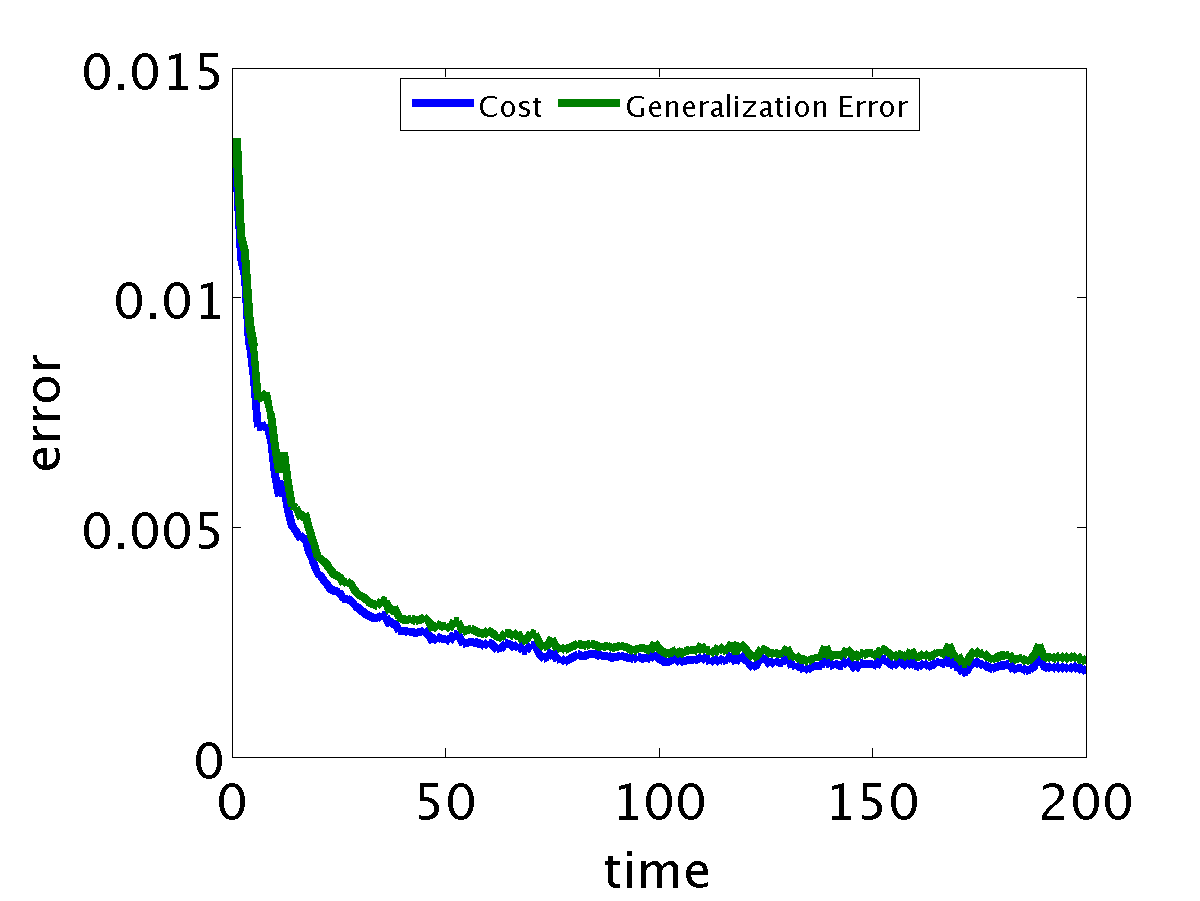
\includegraphics[width=\columnwidth]{./img/errors_train_2000_test_2000.png}
	\caption{The cost, shown in blue, and the generalization error, shown in green, of a training set and test set with each 2000 points for each epoch, with $t_{max} = 200$.}
	\label{fig:exp:errors}
\end{figure}

\begin{figure}
	\centering
	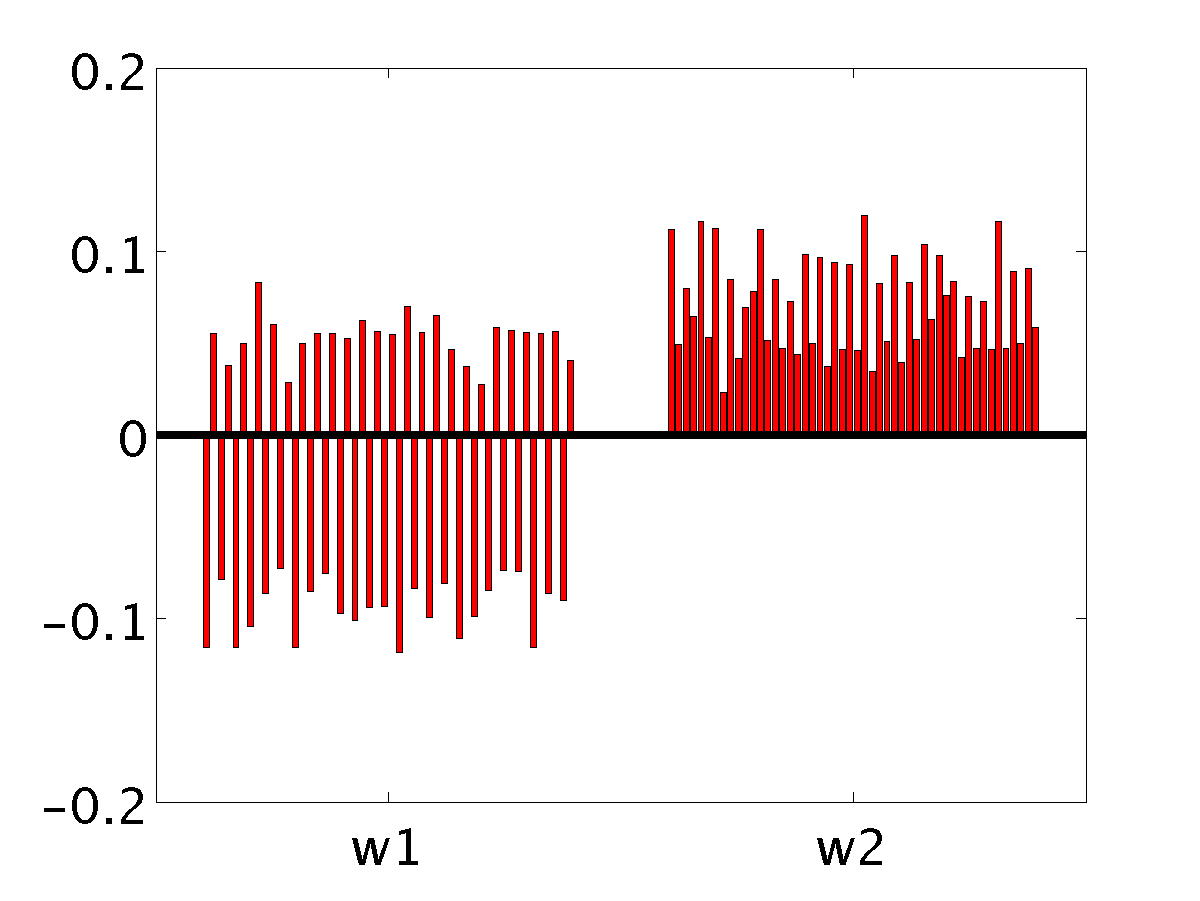
\includegraphics[width=\columnwidth]{./img/weights_train_2000_test_2000.png}
	\caption{The values of the elements of the two weights vectors at $t = 200$.}
	\label{fig:exp:weights}
\end{figure}